\section{Open source licenses and compliance}

\subsection{Introduction}

\begin{frame}{Free software vs. open-source}
  \begin{itemize}
  \item {\bf Free software}: term defined by the {\em Free Software
      Foundation}, grants 4 freedoms
    \begin{itemize}
    \item Freedom to use
    \item Freedom to study
    \item Freedom to copy
    \item Freedom to modify and distribute modified copies
    \item See \url{https://www.gnu.org/philosophy/free-sw.html}
    \end{itemize}
  \item {\bf Open Source}: term defined by the {\em Open Source
      Initiative}, with 10 criterias
    \begin{itemize}
    \item See \url{https://www.opensource.org/docs/osd}
    \end{itemize}
  \item {\em Free Software} movement insists more on ethics, while
    {\em Open Source} insists more on the technical advantages
  \item From a freedom standpoint, they are similar.
  \end{itemize}
\end{frame}

\begin{frame}{Open source licenses}
  \begin{itemize}
  \item All free software/open-source licenses rely on {\em
      copyright law}
  \item Those licenses fall in two main categories
    \begin{itemize}
    \item The copyleft licenses
    \item The non-copyleft licenses, also called {\em permissive}
      licenses
    \end{itemize}
  \end{itemize}
\end{frame}

\begin{frame}{Non-Copyleft VS Copyleft licenses}
  \begin{columns}

    \column{0.5\textwidth}
      \begin{center}
        {\bf Non-Copyleft}\\
        (BSD, MIT, Apache, X11\dots)\\
      {\ }\\
      {\bf You can}\\
      Use\\
      Modify\\
      Redistribute\\
      {\ }\\
      {\bf You must}\\
      Provide license text \\
      Attribution \\
      {\ }
      \end{center}

    \column{0.5\textwidth}
      \begin{center}
        {\bf Copyleft} \\
        (GPL, LGPL, AGPL\dots)\\
      {\ }\\
      {\bf You can}\\
      Use\\
      Modify\\
      Redistribute\\
      {\ }\\
      {\bf You must}\\
      Provide license text \\
      Attribution \\
      Make source code available
       \end{center}

  \end{columns}
\end{frame}

\begin{frame}{What is {\em copyleft}}
  \begin{itemize}
  \item The concept of {\em copyleft} is to ask for reciprocity in the
    freedoms given to a user.
  \item You receive software under a copyleft license and
    redistribute it, modified or not $\rightarrow$ you must do so
    under the same license
    \begin{itemize}
    \item Same freedoms to the new users
    \item Incentive, but no obligation, to contribute back your
      changes instead of keeping them secret
    \end{itemize}
  \item Copyleft is {\em not} the opposite of copyright!
  \item Non-copyleft licenses have no such requirements: modified
    versions can be made proprietary, but they still require
    attribution
  \item \url{https://en.wikipedia.org/wiki/Copyleft}
  \end{itemize}
\end{frame}

\begin{frame}{Open-source licenses in use}
  \begin{columns}
    \column{0.7\textwidth}
    \begin{center}
      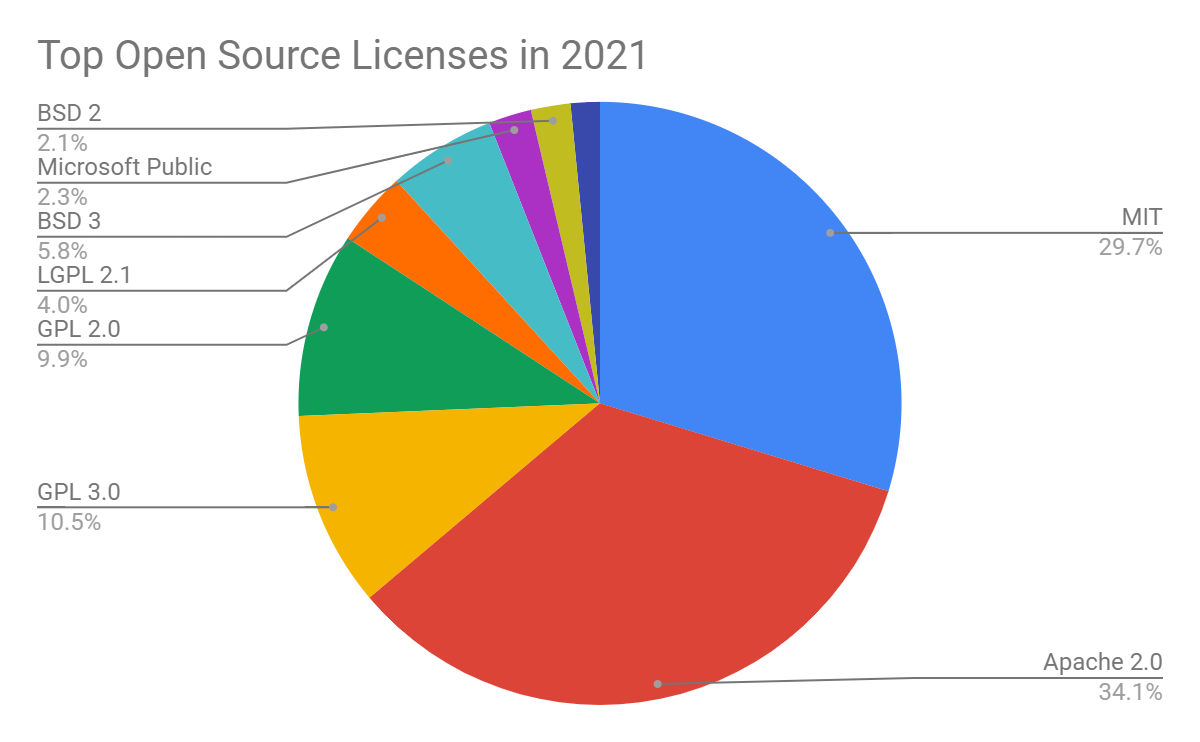
\includegraphics[width=\textwidth]{slides/sysdev-licensing/open-source-licenses-share.png}
    \end{center}
    \column{0.3\textwidth}
    Note: this pie chart is about open-source software in
    general. Your typical embedded Linux system will likely have a
    different proportion of licenses represented.\\
    \vspace{0.5cm}
    Source: \href{https://www.mend.io/resources/blog/open-source-licenses-trends-and-predictions/}{mend.io}
  \end{columns}
\end{frame}

\subsection{Non-copyleft licenses}

\begin{frame}[fragile]{MIT}
  \begin{columns}
    \column{0.45\textwidth}
    \begin{itemize}
    \item Simple permissive license
    \item Widely used
    \item You can do pretty much all what you want, as long as you
      preserve the copyright notice
    \item \url{https://en.wikipedia.org/wiki/MIT_License}
    \end{itemize}
    \column{0.55\textwidth}
    \begin{block}{}
      {\tiny
\begin{verbatim}

Copyright <YEAR> <COPYRIGHT HOLDER>

Permission is hereby granted, free of charge, to any person obtaining
a copy of this software and associated documentation files (the
"Software"), to deal in the Software without restriction, including
without limitation the rights to use, copy, modify, merge, publish,
distribute, sublicense, and/or sell copies of the Software, and to
permit persons to whom the Software is furnished to do so, subject to
the following conditions:

The above copyright notice and this permission notice shall be
included in all copies or substantial portions of the Software.

THE SOFTWARE IS PROVIDED "AS IS", WITHOUT WARRANTY OF ANY KIND,
EXPRESS OR IMPLIED, INCLUDING BUT NOT LIMITED TO THE WARRANTIES OF
MERCHANTABILITY, FITNESS FOR A PARTICULAR PURPOSE AND
NONINFRINGEMENT. IN NO EVENT SHALL THE AUTHORS OR COPYRIGHT HOLDERS BE
LIABLE FOR ANY CLAIM, DAMAGES OR OTHER LIABILITY, WHETHER IN AN ACTION
OF CONTRACT, TORT OR OTHERWISE, ARISING FROM, OUT OF OR IN CONNECTION
WITH THE SOFTWARE OR THE USE OR OTHER DEALINGS IN THE SOFTWARE.
\end{verbatim}
      }
    \end{block}
  \end{columns}
\end{frame}

\begin{frame}[fragile]{Apache License}
  \begin{columns}
    \column{0.5\textwidth}
    \begin{itemize}
    \item Slightly more complex permissive license
    \item Must preserve a \code{NOTICE} file
    \item Includes a {\em patent grant}, a mechanism to prevent users of
      the licensed project from suing others based on patents related to the
      project
    \item \url{https://en.wikipedia.org/wiki/Apache_License}
    \item \url{https://www.apache.org/licenses/LICENSE-2.0}
    \end{itemize}
    \column{0.5\textwidth}
    \begin{block}{}
      {\tiny
\begin{verbatim}
 Apache License
Version 2.0, January 2004
http://www.apache.org/licenses/

TERMS AND CONDITIONS FOR USE, REPRODUCTION, AND DISTRIBUTION

1. Definitions [...]

2. Grant of Copyright License [...]

3. Grant of Patent License [...]

4. Redistribution [...]

5. Submission of Contributions [...]

6. Trademarks [...]

7. Disclaimer of Warranty [...]

8. Limitation of Liability [...]

9. Accepting Warranty or Additional Liability [...]
\end{verbatim}
      }
    \end{block}
  \end{columns}
\end{frame}

\begin{frame}[fragile]{BSD 2 Clause}
  \begin{columns}
    \column{0.45\textwidth}
    \begin{itemize}
    \item Simple permissive license
    \item Not far from the MIT license
    \item Requires preserving a copyright notice
    \item \url{https://opensource.org/licenses/BSD-2-Clause}
    \item \url{https://en.wikipedia.org/wiki/BSD_licenses}
    \end{itemize}
    \column{0.55\textwidth}
    \begin{block}{}
      {\tiny
\begin{verbatim}
Copyright <YEAR> <COPYRIGHT HOLDER>

Redistribution and use in source and binary forms, with or without
modification, are permitted provided that the following conditions
are met:

1. Redistributions of source code must retain the above copyright
notice, this list of conditions and the following disclaimer.

2. Redistributions in binary form must reproduce the above copyright
notice, this list of conditions and the following disclaimer in the
documentation and/or other materials provided with the distribution.

THIS SOFTWARE IS PROVIDED BY THE COPYRIGHT HOLDERS AND CONTRIBUTORS
"AS IS" AND ANY EXPRESS OR IMPLIED WARRANTIES, INCLUDING, BUT NOT
LIMITED TO, THE IMPLIED WARRANTIES OF MERCHANTABILITY AND FITNESS FOR
A PARTICULAR PURPOSE ARE DISCLAIMED. IN NO EVENT SHALL THE COPYRIGHT
HOLDER OR CONTRIBUTORS BE LIABLE FOR ANY DIRECT, INDIRECT, INCIDENTAL,
SPECIAL, EXEMPLARY, OR CONSEQUENTIAL DAMAGES (INCLUDING, BUT NOT
LIMITED TO, PROCUREMENT OF SUBSTITUTE GOODS OR SERVICES; LOSS OF USE,
DATA, OR PROFITS; OR BUSINESS INTERRUPTION) HOWEVER CAUSED AND ON ANY
THEORY OF LIABILITY, WHETHER IN CONTRACT, STRICT LIABILITY, OR TORT
(INCLUDING NEGLIGENCE OR OTHERWISE) ARISING IN ANY WAY OUT OF THE USE
OF THIS SOFTWARE, EVEN IF ADVISED OF THE POSSIBILITY OF SUCH DAMAGE.
\end{verbatim}
      }
    \end{block}
  \end{columns}
\end{frame}

\begin{frame}[fragile]{BSD 3 Clause}
  \begin{columns}
    \column{0.45\textwidth}
    \begin{itemize}
    \item Variant of the BSD 2 Clause license
    \item Includes a {\em non-endorsement} clause
    \item \url{https://opensource.org/licenses/BSD-3-Clause}
    \item \url{https://en.wikipedia.org/wiki/BSD_licenses}
    \end{itemize}
    \column{0.55\textwidth}
    \begin{block}{}
      {\tiny
\begin{verbatim}
Copyright <YEAR> <COPYRIGHT HOLDER>

Redistribution and use in source and binary forms, with or without
modification, are permitted provided that the following conditions are
met:

1. Redistributions of source code must retain the above copyright
notice, this list of conditions and the following disclaimer.

2. Redistributions in binary form must reproduce the above copyright
notice, this list of conditions and the following disclaimer in the
documentation and/or other materials provided with the distribution.

3. Neither the name of the copyright holder nor the names of its
contributors may be used to endorse or promote products derived from
this software without specific prior written permission.

THIS SOFTWARE IS PROVIDED BY THE COPYRIGHT HOLDERS AND CONTRIBUTORS
"AS IS" AND ANY EXPRESS OR IMPLIED WARRANTIES, INCLUDING, BUT NOT
LIMITED TO, THE IMPLIED WARRANTIES OF MERCHANTABILITY AND FITNESS FOR
A PARTICULAR PURPOSE ARE DISCLAIMED. IN NO EVENT SHALL THE COPYRIGHT
HOLDER OR CONTRIBUTORS BE LIABLE FOR ANY DIRECT, INDIRECT, INCIDENTAL,
SPECIAL, EXEMPLARY, OR CONSEQUENTIAL DAMAGES (INCLUDING, BUT NOT
LIMITED TO, PROCUREMENT OF SUBSTITUTE GOODS OR SERVICES; LOSS OF USE,
DATA, OR PROFITS; OR BUSINESS INTERRUPTION) HOWEVER CAUSED AND ON ANY
THEORY OF LIABILITY, WHETHER IN CONTRACT, STRICT LIABILITY, OR TORT
(INCLUDING NEGLIGENCE OR OTHERWISE) ARISING IN ANY WAY OUT OF THE USE
OF THIS SOFTWARE, EVEN IF ADVISED OF THE POSSIBILITY OF SUCH DAMAGE.
\end{verbatim}
      }
    \end{block}
  \end{columns}
\end{frame}

\subsection{Copyleft licenses}

\begin{frame}{GPL: GNU General Public License}
  \begin{itemize}
  \item The flagship license of the GNU project
  \item Used by Linux, BusyBox, U-Boot, Barebox, GRUB, many projects from GNU
  \item Is a copyleft license
    \begin{itemize}
    \item Requires derivative works to be released under the same
      license
    \item Source code must be redistributed, including modifications
    \item If GPL code is integrated in your code, your code must now
      be GPL-licensed
    \item Only applies when redistribution takes place
    \end{itemize}
  \item Also called {\bf strong} copyleft license
    \begin{itemize}
    \item Programs linked with a library released under the GPL must
      also be released under the GPL
    \item Does not prevent GPL programs and non-GPL programs from
      co-existing in the same system or to communicate
    \end{itemize}
  \item \url{https://www.gnu.org/licenses/gpl-2.0.en.html}
  \item \url{https://www.gnu.org/licenses/gpl-3.0.en.html}
  \item \url{https://en.wikipedia.org/wiki/GNU_General_Public_License}
  \end{itemize}
\end{frame}

\begin{frame}{LGPL: GNU Lesser General Public License}
  \begin{itemize}
  \item Used by {\em glibc}, {\em uClibc}, and many libraries
  \item Derived from the GPL license
  \item Also a copyleft license
  \item But a {\bf weaker} copyleft license
    \begin{itemize}
    \item Programs linked against a library under the LGPL do not need
      to be released under the LGPL and can be kept proprietary.
    \item However, the user must keep the ability to update the
      library independently from the program.
    \item Requires using dynamic linking, or in the case of static
      linking, to provide the object files to relink with the library
    \end{itemize}
  \item \url{https://www.gnu.org/licenses/lgpl-2.1.en.html}
  \item \url{https://www.gnu.org/licenses/lgpl-3.0.en.html}
  \item
    \url{https://en.wikipedia.org/wiki/GNU_Lesser_General_Public_License}
  \end{itemize}
\end{frame}

\begin{frame}{GPL/LGPL: redistribution}
  \begin{itemize}
  \item No obligation when the software is not distributed
    \begin{itemize}
    \item You can keep your modifications secret until the product
      delivery
    \end{itemize}
  \item It is then authorized to distribute binary versions, if one of
    the following conditions is met:
    \begin{itemize}
    \item Convey the binary with a copy of the source on a physical
      medium
    \item Convey the binary with a written offer valid for 3 years
      that indicates how to fetch the source code
    \item Convey the binary with the network address of a location
      where the source code can be found
    \end{itemize}
  \item In all cases, the attribution and the license must be
    preserved
  \end{itemize}
\end{frame}

\begin{frame}{GPL/LGPL: version 2 vs version 3}
  \begin{itemize}
  \item GPLv2/LGPLv2 published in 1991, widely used in the open-source
    world for major projects
  \item GPLv3/LGPLv3 published in 2007, and adopted by some projects
  \item Main differences
    \begin{itemize}
    \item More {\em legalese} and definitions to clarify the license
    \item Explicit patent grant
    \item Grace period of 30 days to get back into compliance instead
      of immediate termination
    \item Anti-Tivoization clause
    \end{itemize}
  \item Anti-Tivoization
    \begin{itemize}
    \item Requirement that the user must be able to {\bf run} the
      modified versions on the device
    \item Need to provide {\em installation instructions}
    \item Only required for {\em User products}, i.e. consumer devices
    \item On-going debate on how strong this requirement is, and how
      difficult it is to comply with
    \end{itemize}
  \end{itemize}
\end{frame}

\begin{frame}{GPL: v2, v3, v2 or later, v3 or later}
  \begin{itemize}
  \item Some projects are released under {\em GPLv2 only}
    \begin{itemize}
    \item Examples: Linux kernel, U-Boot
    \end{itemize}
  \item Some projects are released under {\em GPLv3 only}
  \item Some projects are released under {\em GPLv2 or later}
    \begin{itemize}
    \item The recipient can chose to apply either the terms of GPLv2,
      GPLv3 or any later version
    \end{itemize}
  \item Some projects are released under {\em GPLv3 or later}
    \begin{itemize}
    \item The recipient can chose to apply the terms of GPLv3 or any
      later version (none of which exists today)
    \item Examples: GCC, Samba, Bash, GRUB
    \end{itemize}
  \item Note: this logic applies similarly to the LGPL license.
  \end{itemize}
\end{frame}

\begin{frame}{Dual licensing}
  \begin{itemize}
  \item Some companies use a {\em dual licensing} business model,
    mainly for software libraries
  \item Their software is offered under two licenses:
    \begin{itemize}
    \item A strong copyleft license, typically GPL, to encourage
      adoption of the software by the open-source world, allow the
      development and distribution of GPL licensed applications based
      on this library
    \item A commercial license, offered against a fee, which allows to
      develop and distribute proprietary applications based on this
      library.
    \end{itemize}
  \item Examples: Qt (only parts), MySQL, wolfSSL, Asterisk, etc.
  \end{itemize}
\end{frame}

\begin{frame}
  \frametitle{Is this free software?}
  \begin{itemize}
  \item Most of the free software projects are covered by about 10
    well-known licenses, so it is fairly easy for the majority of
    projects to get a good understanding of the license
  \item Check Free Software Foundation's opinion\\
    \url{https://www.fsf.org/licensing/licenses/}
  \item Check Open Source Initiative's opinion\\
    \url{https://www.opensource.org/licenses}
  \item Otherwise, read the license text
  \end{itemize}
\end{frame}

\begin{frame}{Licensing: examples}
  \begin{center}
    \includegraphics[width=\textwidth]{slides/sysdev-licensing/license-cases.pdf}
  \end{center}
\end{frame}

\subsection{Best practices}

\begin{frame}{Respect free software licenses}
  \begin{itemize}
  \item Free Software is not public domain software, the distributors
    have obligations due to the licenses
  \item {\bf Before} using a free software component, make sure the
    license matches your project constraints
  \item Make sure to keep your modifications and adaptations
    well-separated from the original version.
  \item Make sure to keep a complete list of the free software
    packages you use, and the version in use
  \item Buildroot and Yocto Project can generate this list for you!
    \begin{itemize}
    \item Buildroot: \code{make legal-info}
    \item Yocto: see
      \href{https://docs.yoctoproject.org/dev-manual/common-tasks.html\#maintaining-open-source-license-compliance-during-your-product-s-lifecycle}{the
        project documentation}
    \end{itemize}
  \item Conform to the license requirements before shipping the
    product to the customers.
  \end{itemize}
\end{frame}

\begin{frame}{Keeping changes separate}
  \begin{itemize}
  \item When integrating existing open-source components in your
    project, it is sometimes needed to make modifications to them
    \begin{itemize}
    \item Better integration, reduced footprint, bug fixes, new
      features, etc.
    \end{itemize}
  \item Instead of mixing these changes, it is much better to keep
    them separate from the original component version
    \begin{itemize}
    \item If the component needs to be upgraded, easier to know what
      modifications were made to the component
    \item If support from the community is requested, important to
      know how different the component we're using is from the
      upstream version
    \item Makes contributing the changes back to the community
      possible
    \end{itemize}
  \item It is even better to keep the various changes made on a given
    component separate
    \begin{itemize}
    \item Easier to review and to update to newer versions
    \end{itemize}
  \item Use your favorite version control system and/or stack of
    patches.
  \end{itemize}
\end{frame}
